\fig{fv:w3:beats}{包络的绝对值给振幅，负包络对应快振动相位翻转}{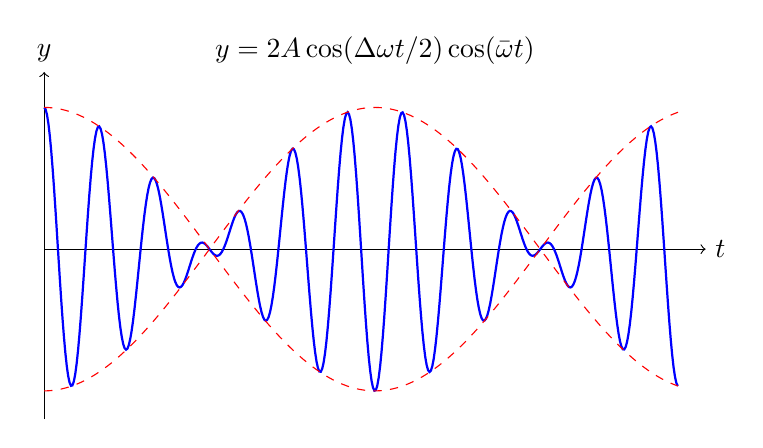
\begin{tikzpicture}[x=.7cm,y=.9cm]
\draw[->](0,0)--(12,0)node[right]{$t$};\draw[->](0,-2.4)--(0,2.5)node[above]{$y$};
\draw[blue,thick,domain=0:11.5,samples=450]plot(\x,{2*cos(30*\x)*cos(360*\x)});
\draw[red,dashed,domain=0:11.5,samples=150]plot(\x,{2*cos(30*\x)});
\draw[red,dashed,domain=0:11.5,samples=150]plot(\x,{-2*cos(30*\x)});
\node at(6,2.8){$y=2A\cos(\Delta\omega t/2)\cos(\bar\omega t)$};\end{tikzpicture}}
图\ref{fv:w3:beats}中慢变因子过零后可以变负，但可观测振幅是 $2A|\cos(\Delta\omega t/2)|$，不取负值。相邻两次强度最强的间隔因此为 $2\pi/|\Delta\omega|$，拍频为 $|f_1-f_2|$；若把不取绝对值的余弦周期直接当成拍周期，就会多一个二。两频率相差远小于平均频率时，才容易分辨快振动与慢包络。
